\documentclass[letterpaper]{article}
%\usepackage{../../../LaTeX/styles/aaai}
\usepackage{aaai}
\usepackage{times}
\usepackage{helvet}
\usepackage{courier}
\usepackage{latexsym} 
\usepackage{graphicx}
\usepackage{algorithm}
\usepackage{algorithmic}
\usepackage{url}
\usepackage{colortbl}
\usepackage{color}
\usepackage{subfigure}
\usepackage{amsmath}
\usepackage{amssymb}
\usepackage{enumerate}
\usepackage[belowskip=-5pt,aboveskip=5pt]{caption}

\newtheorem{df}{Definition}
\newtheorem{notation}{Notation}
\newtheorem{theorem1}{Theorem}
\newtheorem{theorem}{Theorem}
\newtheorem{lemma}{Lemma}[section]
\newtheorem{col}{Corollary}
\newcommand{\bt}{\begin{theorem}\em}
\newcommand{\et}{\end{theorem}}
\newcommand{\Qed}{$\blacksquare$}
\newcommand{\qed}{$\Box$}
\newcommand{\proof}{{\bf Proof. }}

\newcommand{\nin}{\noindent}

\setlength{\intextsep}{10pt plus 2pt minus 2pt}

\newcommand{\bea}{\begin{eqnarray}}
\newcommand{\eea}{\end{eqnarray}}

\newcommand{\bdf}{\begin{df}\em}
\newcommand{\edf}{\end{df}}

\newcommand{\ben}{\begin{enumerate}}
\newcommand{\een}{\end{enumerate}}
\newcommand{\ie}{\item}

\newcommand{\dist}{\operatorname{dist}}

\newcommand{\avg}{\operatorname{avg}}

\definecolor{grey}{rgb}{0.4,0.4,0.4}


\numberwithin{equation}{section}
\numberwithin{theorem}{section}
\numberwithin{lemma}{section}
\numberwithin{df}{section}

\title{Drafting Territories in the Board Game Risk\\ Submission \#}

\nocopyright

\author{Author(s) Name(s) Go Here in 12 Point Bold Times Type}
%\author{Neesha Desai, Richard Gibson, and Richard Zhao \\
%Department of Computing Science, University of Alberta \\
%Edmonton, Alberta, T6G 2E8, Canada \\
%$\{$neesha$\mid$rggibson$\mid$rxzhao$\mid$bulitko$\}$@cs.ualberta.ca}


\begin{document}

\maketitle

\begin{abstract}
In the standard rules of the board game Risk, players take turns selecting or ``drafting'' the 42 territories on the board until all territories are owned.  We present a technique for drafting territories in Risk that combines the Monte Carlo tree search algorithm UCT with an automated evaluation function.  Created through supervised machine learning, this function scores outcomes of drafts in order to shorten the length of a UCT simulation.  Using this approach, we augment an existing bot for the computer game Lux Delux, a clone of Risk.  Our drafting technique is shown to greatly improve performance against the strongest opponents supplied with Lux Delux.  The evidence provided indicates that territory drafting is important to overall success in Risk.
\end{abstract}

\section{Introduction}

% Talk about search for single agent, minimax for two-player, 0-sum, max$^\text{n}$ for multi-player.  Examples like chess, checkers, etc.

For the past few decades, computer games have been a popular platform for artificial intelligence research.  Many successful computer programs (bots) play at expert levels in two-player games such as checkers \cite{Chinook}, Othello \cite{Othello}, and
chess \cite{DeepBlue}.  These are popular two player games where both players share complete information about the game states.  Such games are handled well by classical minimax search with alpha-beta pruning and some evaluation function (often hand-tuned) for intermediate states.  

However, games involving more than two players (multi-player) are generally less understood.  In this paper, we describe how to create stronger bots for playing the multi-player game Risk by Hasbro Inc.  In the standard rules of Risk, the game begins with the players drafting the territories on the board until every territory has an owner.  Our work here focuses on improving overall performance by developing an intelligent system for playing the opening territory draft phase of Risk.

The rest of the paper is organized as follows.  First, we provide an outline for the rules of Risk.  Second, we discuss related work, including traditional minimax search, its extension to multi-player games, max$^\text{n}$, and the Monte-Carlo tree search algorithm UCT.  We then describe how our system drafts territories in Risk.  Our approach combines UCT with a machine-learned evaluation function to search the game tree up to the end of the drafting phase, where an estimate of the merits of the draft outcomes are propagated back.  Next, using a computer version of Risk, we create a bot that uses our drafting technique and pit it against a number of others programs.  The empirical results show that our bot outperforms all of its opponents, even those using post-draft strategies identical to our own.  This suggests that the drafting phase is a very meaningful part of Risk.  Finally, we summarize the results and conclude with some future works.

\section{Risk}
\label{sec:Prob}

% Rules of Risk, particularly the drafting stage
Risk is a strategy board game for two to six players where the objective is to occupy all 42 territories on the board.  The territories are divided into 6 continents as labelled in Figure \ref{fig:Conts}.  In the standard rules, players first take turns selecting the territories until all have been chosen.  After players place their initial armies among their selected territories, players then take turns until only one player remains.  On a turn, in sequence a player may place reinforcements, conduct attacks on opposing territories, and tactically maneuver armies amongst owned territories.  Attacks are resolved by dice rolls, where the number of dice is dependent on the number of attacking and defending armies.  A player reduced to zero armies on the board is eliminated from the game.  Players receive one reinforcement army for every three territories owned, and receive bonus reinforcements for owning entire continents (as depicted in Figure~\ref{fig:Conts}). %or trading in cards earned by conquering territories. 
Full rules can be found on-line \cite{Risk}.

\begin{figure}[t]
	\centering
	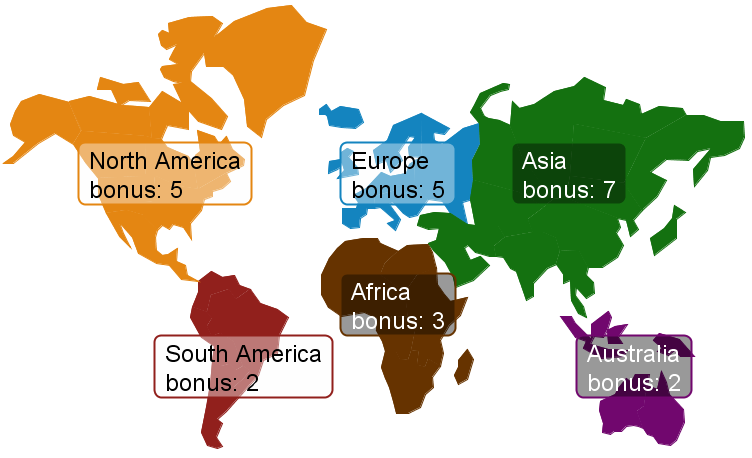
\includegraphics[scale=0.325]{../ForPublication/figs/Conts.png}
	\caption{The layout of the Risk board and the continent reinforcement bonuses.}
	\label{fig:Conts}
\end{figure}

The Lux Delux (Sillysoft 2010) \nocite{Lux} %\cite{Lux} %(Sillysoft 2010)  %\footnote{http://sillysoft.net/lux/} 
game is a commercialized computer version of Risk, providing several rule-based bots with source code to play against.  Each of the included bots has an associated difficulty and a general playing style.  For example, ``Quo'' is a difficult bot that tries to form a cluster of adjacent territories and methodically expand that cluster.  We use the Lux Delux environment in all of our computations and experiments.  

In this paper, we are only concerned with strategies for playing the opening territory selection phase of Risk.  In addition, we focus only on three player Risk, as this incorporates the multi-player aspect and is arguably more strategically demanding compared to playing with more players.  With fewer players, each player must make more selections in the opening draft.  Since we are only concerned with playing the opening draft of Risk, we simply use the Quo bot's rules for our own post-draft play. 

\section{Related Work}

A widely known approach to game playing is the minimax adversarial search algorithm.  It is designed for zero-sum games involving two players, denoted Max and Min.  The Max player (assumed to be the active player) performs a search of a game tree rooted at the current state of the game.  Each leaf node of the tree is evaluated by a heuristic function, which returns a value estimating the merit of the state to Max.  These values are then backed up the tree; at nodes belonging to Max, the maximum value of the children is propagated up, whereas at nodes belonging to Min, the minimum value of the children is used.  The Max player then chooses the action at the root leading to the child with the maximum propagated value.

% max$^\text{n}$, Paranoid
% MP-Mix which extends max$^\text{n}$ (was used only for branching factor of 3, and for single winner games)

While minimax search is traditionally employed in many two-player games, it is not applicable to games with $n > 2$ players.  A generalization of traditional minimax search to more players is the max$^\text{n}$ algorithm \cite{MaxN}.  At the leaf nodes of the game tree, a heuristic function now estimates a vector of $n$ merits $(v_1, ..., v_n)$, one for each player.  At nodes belonging to player $i$, the vector with the highest merit $v_i$ is propagated up to the parent.  Thus, players are assumed to be maximizing their own individual payoffs throughout the remainder of the game.  An alternative to max$^\text{n}$ is the Paranoid algorithm \cite{Paranoid}, where the active player assumes that the other players are out to minimize his or her payoff with complete disregard to their own benefits.  The Paranoid algorithm is essentially equivalent to the minimax algorithm, where the other players are represented as one meta-player (Min) attempting to minimize the individual heuristic value of the active player (Max).  Finally, the max$^\text{n}$ and Paranoid propagation strategies can be dynamically selected according to the game situation.  This is done in the MP-Mix algorithm \cite{ZuckFelnerKraus2009}, along with a third strategy called Offensive.  On the whole, these algorithms perform best when the branching factor (i.e.~action space) is small and when there exists a good evaluation function for approximating the merits of non-terminal states.  Unfortunately, when drafting in Risk the first player has 42 actions to choose from initially, and we know of no such evaluation function to use for territory selection.

%\begin{algorithm}[t]
%	\caption{max$^\text{n}$+UCT($s$, $d$, $M$, $c$)}
%	\label{alg:maxNUct}
%	\begin{footnotesize}
%	\begin{algorithmic}[1]
%		\IF{$s$ is terminal}
%			\RETURN $\cdot$, vector of values of $s$ to each player
%		\ENDIF
%		\STATE Run UCT($c$) simulations from $s$ until $s$ has been visited $M$ times, obtaining $\vec{Q}(s,a)$ for all actions $a$ at $s$
%		\STATE $i \gets $ Player to act at $s$
%		\STATE $(a_1, a_2, ...) \gets $ Actions at $s$ sorted by decreasing $Q_i(s,a)$
%		\IF{$d = 0$ OR $s$ is terminal}
%			\RETURN{$a_1, \vec{Q}(s,a_1)$}
%		\ENDIF
%		\STATE $b \gets $ number of turns $i$ has in next $d$ moves
%		\FOR{$k$ from $1$ to $b$}
%			\STATE $s' \gets $ NextState($s, a_k$)
%			\STATE $\cdot, \vec{V}^k \gets $ max$^\text{n}$+UCT($s'$, $d - 1$, $M$)
%		\ENDFOR
%		\STATE $k^* \gets \text{argmax}_k V_i^k$
%		\RETURN{$a_{k^*}, \vec{V}^{k^*}$}
%	\end{algorithmic}
%	\end{footnotesize}
%\end{algorithm}

An algorithm more suited for large actions spaces and requiring no evaluation function is UCT \cite{UCT}, a Monte Carlo planning algorithm that has been used effectively in Computer Go \cite{ComputerGo} and general game playing, for example in CadiaPlayer \cite{Cadia}.  UCT tries to intelligently bias the game tree by simulating games that focus on appealing branches of the tree.  At each step, UCT builds upon the sparse game tree from the previous simulations by selecting an action $a$ at state $s$ to expand by
\[ a = \text{argmax}_{a'} \left( Q_i(s,a') + c \sqrt{ \log n(s) / n(s,a') } \right), \]
where $Q_i(s,a)$ is the estimated value for player $i$ of taking $a$ at $s$, $i$ is the active player at $s$, $c$ is an exploration constant, $n(s)$ is the number of times $s$ has been visited, and $n(s,a)$ is the number of times $a$ has been taken in $s$.  The estimate $Q_i(s,a)$ is equal to the average final game value player $i$ received on previous simulations where $s$ was visited and $a$ was taken at $s$.  This final game value is typically 1 for a win and 0 for a loss in win-lose type games.  On each simulation, UCT adds one new node to the game tree and then randomly plays out the rest of the game.  After running numerous simulations from the current state $s$, UCT takes the action $\text{argmax}_{a}Q_i(s,a)$.

We now describe some previous work related to drafting territories in Risk.  One related area is the problem of drafting athletes in sports leagues, to which some progress has been made.  Many professional sports use a drafting procedure where teams sequentially select entry-level players based on the teams' current needs and scouting reports of the players' skills.  Brams and Straffin \cite{PrisonAndDrafting} examine very small games where each team has its own order of preference of the entering players.  They use a max$^\text{n}$-type approach to find optimal drafting strategies, but hint that the approach is ill-advised for larger drafts due to a prohibitively large branching factor.  In addition, Fry et.~al \cite{SportsDrafting} solve a deterministic dynamic programming problem through linear programming to determine a team's best drafting strategy and apply it to a fantasy football draft.  However, a key ingredient in their model is that each team has positional (quarterback, running back, etc.) needs and must limit its picks to a fixed number of players for each position.  For Risk drafting, we are not concerned with restricting territories to competitors in any way.

Finally, playing Risk in particular has garnered some attention from the AI community.  Firstly, the program MARS \cite{RiskBots} is a multi-agent system for Risk that deploys an agent in each territory on the board.  The system's actions for placing armies, conducting attacks, and fortifying territories are determined through ``bids" submitted by the territory agents.  These bids evaluate the territories via hand-tuned features and parameter values.  Secondly, Zuckerman, Felner, and Kraus used Risk as a testbed for their MP-Mix algorithm \cite{ZuckFelnerKraus2009}.  To do so, they restricted the branching factor to only 3 promising moves, where a move represented an entire sequence of territories to conquer.  However, both of these approaches use a Risk variant where territories are randomly assigned to begin the game rather than selected by the players.  We are not aware of any previous work regarding the drafting phase of Risk.

\section{Our Approach}

%\begin{figure*}[t]
%	\centering
%	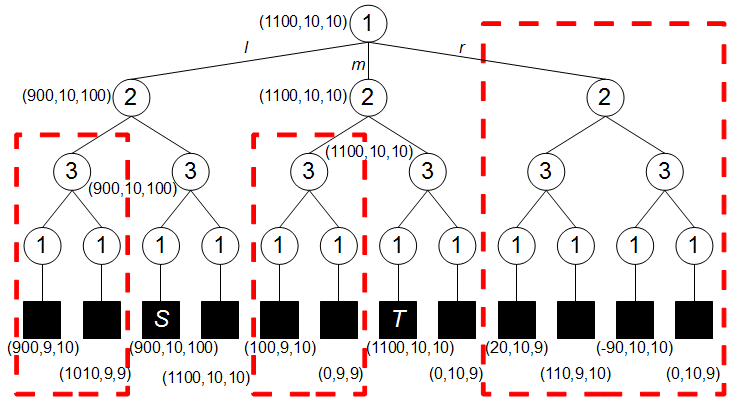
\includegraphics[scale=0.75]{../ForPublication/figs/MaxNExample.png}
%	\caption{An example game tree involving 3 players.  Numbered circles represent player decision points and black squares indicate terminal nodes, with the values of the terminal node to each player staggered below.}
%	\label{fig:MaxNEx}
%\end{figure*}

%For drafting territories in Risk, we use a hybrid of both the max$^\text{n}$ algorithm and UCT.  Since max$^\text{n}$ is not very practical when there are many possible actions and no known evaluation functions, we use UCT to both restrict the branching factor and evaluate non-terminal positions in the max$^\text{n}$ tree.  In addition, rather than simulating entire Risk games, we instead derive scores for draft outcomes using supervised machine learning for UCT to pass back up the tree.  We now describe our hybrid algorithm and the score derivation technique below.

%\subsection{Combining max$^\text{n}$ and UCT}
%
%% Intuition as to why it might be better than UCT
%Let's assume that we have some fixed time limit $t$ to take an action.  When trying to decide which action to take at the root node of a game tree, UCT runs as many simulations from the root as possible in $t$ units of time.  This results in a lot of visits to nodes near the root of the tree, providing a thorough estimate of the value of each of these states.  However, on average, nodes deeper in the tree are visited fewer times because each simulation takes a single path through the game tree.  Rather than spending all of this time evaluating the root, we may be able to make a more informed decision if we have a better estimate of the future moves we and our opponents might later take.  Our algorithm distributes the simulations not only at the root of the tree, but also at deeper nodes along promising lines of play.
%
%% Walk through the lines of the algorithm
%
%The hybrid max$^\text{n}$+UCT algorithm is provided in Algorithm \ref{alg:maxNUct}.  The method is recursive and is called by passing in the current state $s$, a maximum depth (or lookahead horizon) $d$, a limit $M$ on the number of UCT simulations to run per function call, and a UCT exploration constant $c$.  First, UCT simulations are run from $s$ until a total of $M$ simulations have passed through $s$, including simulations from prior function calls from this turn and previous turns (line 4).  Then, the possible actions are sorted from best to worst according to the value of each action to the active player, $Q_i(s,a)$, provided by the $M$ UCT simulations (line 6).  If we have reached our depth limit, then the most promising action $a_1$ is returned, along with the values of that action to each player, $\vec{Q}(s,a_1)$ (line 8).  Otherwise, we continue with the max$^\text{n}$ portion of the algorithm by expanding the $b$ most promising moves, where $b$ is the number of moves the active player has remaining in our lookahead horizon (line 10).  In Risk, players take turns in sequence, and so for 3-player Risk drafting $b = \left\lceil \frac{d + 1}{3} \right\rceil$.  For each expanded action $a_k$, we obtain the value of that action to each player, $\vec{V}^k$, by recursively calling max$^\text{n}$+UCT on the next state with a decremented horizon (line 13).  Finally, the top-valued action to the active player $a_{k^*}$ among the expanded actions is returned, along with the value of $a_{k^*}$ to each player, $\vec{V}^{k^*}$ (line 16).  The action $a_{k^*}$ returned by the original call to max$^\text{n}$+UCT is the action taken in the game.
%
%% Example that we can talk about both here and when we first mention max^n?
%
%Consider the example game tree in Figure \ref{fig:MaxNEx} where players 1 (the active player), 2, and 3 must each take an action in turn, followed by a final forced action by player 1.  Note that the average payouts for player 1 at the 4 terminal nodes below branch $m$ (300) are much less than those under branch $l$ (977.5).  However, assuming players 2 and 3 play optimally, the correct choice for player 1 is to play $m$ for an eventual value of 1100 rather than $l$ for 900.  Because UCT plays randomly at initial visits to nodes and explores according to the parameter $c$, it will likely take many simulations for the average payouts passing through $m$ to be greater than those passing through $l$.  For example, with a small exploration constant $c$, unless the first simulation through $m$ happens to follow the path to the terminal node labelled $T$, future simulations from the root will avoid $m$ for some time.  If $c$ is too large, each of $l$, $m$, and $r$ will be explored roughly equally to start and the early estimates will approximately be the average payouts of the terminal nodes beneath them. In either case, $l$ will incorrectly appear to be the better choice to UCT until enough simulations are run.  
%
%
\begin{figure*}[t]
	\centering
	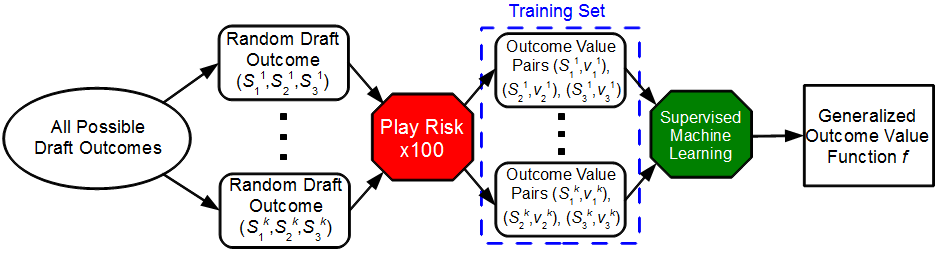
\includegraphics[scale=0.5]{../ForPublication/figs/MachineLearner.png}
	\caption{The process described for obtaining a general function $f$ for estimating the merit of each feature set in Risk draft outcomes (adapted from \cite[Figure 5.1]{GregLeeThesis}).}
	\label{fig:MachLearn}
\end{figure*} 
%
%Let's now walk through an application of max$^\text{n}$+UCT to the example in Figure \ref{fig:MaxNEx} with maximum depth $d = 4$.  First, $M$ UCT simulations are run from the root, providing estimates of the 3 possible actions $l$, $m$, and $r$.  Assuming the estimate for $r$ is the lowest, max$^\text{n}$+UCT then effectively cuts off this branch from the search (as indicated in Figure \ref{fig:MaxNEx} by the dashed red box) as player 1 has only 2 actions remaining.  Next, in a depth-first ordering, at most $M$ simulations are run from each of the two remaining nodes for player 2, and similarly the branch with the lowest estimate is cut off (as this is players 2's last action).  At most $M$ simulations are also run at the two remaining player 3 nodes and again the sub-branch with the lowest estimate is cut (the red boxes are omitted for these two cuts).  Finally, by making a trivial modification so that no UCT simulations are run at nodes with only 1 action, we reach the two terminal nodes labelled $S$ and $T$.  The value of these two nodes are passed back up the tree, and we now take action $m$ at the root as it leads to the highest value for player 1.  With enough exploration, only a small number of simulations $M$ need to be performed at each of the 5 nodes to achieve this result with max$^\text{n}$+UCT.  As mentioned above, if $M$ is small, UCT will likely decide to take action $l$ after only $5M$ simulations.
%
%The depth parameter $d$ allows max$^\text{n}$+UCT to be used in time-constrained scenarios by making repeated calls and iteratively increasing $d$, much like in the single-agent search algorithm IDA$^*$ \cite{IdaStar}.  For Risk drafting, we start with $d = 0$ and increase $d$ by the number of players, 3, after each completion of the algorithm.  In addition, we found through preliminary experiments that $M = 3000$ provided enough simulations for UCT to provide decent estimates for the values of selecting each territory, and that moderately increasing this number resulted in no significant improvement.  Note that calling max$^\text{n}$+UCT($s$, $0$, $M$, $c$) is equivalent to calling UCT($c$) at $s$ for $M$ simulations.  
%

We use UCT as our main algorithm for drafting territories in Risk, since max$^\text{n}$ and other traditional search algorithms are not practical when there are many possible actions and no known evaluation functions.  One issue with applying UCT simulations, however, is that Risk is not well-suited to numerous runs of the entire game as games typically last a long time.  Furthermore, if all players play randomly in Risk, there is no guarantee that the game will even end.  Since UCT simulates games randomly beyond previously stored states in its search tree, the algorithm is unlikely to complete more than a small number of simulations, leading to poor estimates of the possible actions.  To increase the rate at which simulations can be performed, we instead simulate only the initial drafting portion of the game, which has a fixed length (the number of territories remaining to be selected) regardless of random play.  This is done by evaluating each draft outcome with a numerical score that estimates our probability of winning the entire game of Risk from that draft outcome.  These scores are generated off-line using supervised machine learning, which we now describe.
%
%\subsection{Evaluating Draft Outcomes}

Our learning technique is closely related to Lee's work \cite{GregLeeThesis} of combining single-agent heuristic search with a machine-learned fitness function to pick a set of actions from a large library.  Lee's objective is to find a small set of actions which allow the agent to behave as close to optimal as possible in a Markov decision process, relative to having access to the entire library of actions.  Our approach here can be seen as an extension of Lee's work from a single-agent problem to a competitive multi-agent problem, where we replace single-agent search with an adversarial method, UCT. 

\begin{table*}[t]
 \centering
      \caption{The weights for features of type (i), as computed in Weka.  Rows denote continents and columns denote territory counts.  Weights denoted with a * are derived through linear extrapolation.}
    \label{tab:ContScoring}
    \begin{footnotesize}
    \begin{tabular}{|c|c|c|c|c|c|c|c|c|c|c|c|c|c|}
    	\hline
    	  & \bf 0 & \bf 1 & \bf 2  & \bf 3 & \bf 4 & \bf 5 & \bf 6 & \bf 7 & \bf 8 & \bf 9 & \bf 10 & \bf 11 & \bf 12 \\
    	 \hline
    	\bf Australia & 2.97 & 0 & 8.45 & 9.99 & 10.71 & - & - & - & - & - & - & - & - \\
    	\hline
    	\bf South Amer. & 0.69 & 1.23 & 3.90 & 0 & 17.72 & - & - & - & - & - & - & - & - \\
    	\hline
    	\bf Africa & 14.40 & 12.87 & 10.72 & 7.16 & 1.23 & 0 & 29.80 & - & - & - & - & - & - \\
    	\hline
    	\bf North Amer. & 3.11 & 0.98 & 0 & 2.17 & 7.15 & 19.35 & 24.82 & 24.10 & 36.15 & 48.20* & - & - & - \\
    	\hline
    	\bf Europe & 42.44 & 45.11 & 43.11 & 43.77 & 41.35 & 50.77 & 43.85 & 36.93* & - & - & - & - & - \\
    	\hline
    	\bf Asia & 27.10 & 23.90 & 23.61 & 23.10 & 23.61 & 23.68 & 19.32 & 15.63 & 17.43 & 13.84 & 10.25* & 6.66* & 3.07* \\
    	\hline
    \end{tabular}
    \end{footnotesize}
\end{table*}

We manually identified a number of features that are tactically important in draft outcomes of Risk.  Many of these features are inspired by the calculation of highest ``bids'' \cite{RiskBots}.  For each player, our features are described by: (i) for each continent, the number of territories owned in that continent; (ii) when the player plays in the turn order; (iii) the number of distinct territories owned by other players which border owned territories (enemy neighbors); and (iv) the number of distinct ordered pairs of owned territories which are adjacent (friendly neighbors).  Our process for estimating the merit of a feature set is depicted in Figure \ref{fig:MachLearn}.  First, we collect many draft outcomes, each obtained by randomly assigning all 42 territories evenly among the 3 players.  Then, for each draft outcome, 100 games are played to completion where each player follows the post-draft strategy of the Quo bot provided with the Lux Delux software package.  Each player $i$, $i=1,2,3$, has a set of features $S_i$ associated with each outcome.  Each feature set is assigned a value $v_i \in \{0,1,...,100\}$ equal to the number of games that player $i$ eventually won from the associated draft outcome.  This provides a collection of feature set value pairs $\{(S_i, v_i)\}$ of size equal to three times the number of draft outcomes collected.  Next, supervised machine learning is applied to obtain a general function
\[ f: S \mapsto v \in \textbf{R} \] 
that estimates the merit of the feature set $S$ when following Quo's post-draft strategy.  Finally, for a draft outcome $Z = (A_1,A_2,A_3)$ with $A_i$ being the set of player $i$'s territory selections, we calculate $v_i = f(S_i)$ where $S_i$ is the feature set associated with $A_i$, and define the value of the draft outcome $Z$ for player $i$ to be
\[ V_i(Z) = v_i^+ / \left(v_1^+ + v_2^+ + v_3^+\right), \]
where $v_i^+ = \max(0, v_i)$.  
%Note that even though all training values $v_i$ are nonnegative, a learner could allow $f$ to be negative and so we take the max to ensure $V_i(Z) \in [0,1]$.  
%Thus, $V_i(Z) \in [0, 1]$ approximately measures the value of our selections relative to the picks made by the other players, providing an estimate of player $i$'s chance of winning from $Z$.
Thus, player $i$ attempts to maximize the estimated merit $v_i$ of his or her selections while minimizing those of the opponents.

Our general function $f$ was computed off-line from $7364$ random draft outcomes for a total of $22092$ $(S,v)$ pairs.  We used Weka \cite{Weka} to weight each individual feature using Weka's linear regression classifier (with no attribute selection), where features (i) and (ii) were represented as nominal features and features (iii) and (iv) were numeric.  Thus, $f(S)$ can be calculated by simply summing the weights, displayed in Tables \ref{tab:ContScoring} and \ref{tab:MoreScoring}, of the features present in $S$.  However, there are some features of type (i) which did not appear in any of the $22092$ feature sets because of their unlikeliness of occurring through random drafting; for instance, there were no cases where one player owned all 9 territories of North America.  The weights of these features were calculated through linear extrapolation of the closest two continent counts for the associated continent.  As an example, the weight for owning all 9 territories in North America is calculated from the weights for owning 8 territories and 7 territories in North America via
\[ 36.15 + (36.15 - 24.10) = 48.20. \]  

%\begin{table*}[t]
%  \begin{center} 
%   \caption{The weights for features of type (i), as computed in Weka.  A * denotes weights derived through linear extrapolation.}
%    \label{tab:ContScoring}
%    \begin{tabular}{|c|c|c|c|c|c|c|}
%    	\hline
%    	\bf Number of Territories & \bf Australia & \bf South America & \bf Africa & \bf North America & \bf Europe & \bf Asia \\
%    	\hline
%    	\bf 0 & 2.972 & 0.6904 & 14.3958 & 3.1092 & 42.4404 & 27.0974 \\
%    	\hline
%    	\bf 1 & 0 & 1.232 & 12.8728 & 0.9766 & 45.1071 & 23.9027 \\
%    	\hline
%    	\bf 2 & 8.4532 & 3.8997 & 10.7207 & 0 & 43.1116 & 23.6086 \\
%    	\hline
%    	\bf 3 & 9.9902 & 0 & 7.1637 & 2.1682 & 43.7726 & 23.1026 \\
%    	\hline
%    	\bf 4 & 10.7097 & 17.7184 & 1.23 & 7.1541 & 41.3515 & 23.6086 \\
%    	\hline
%    	\bf 5 & - & - & 0 & 19.3505 & 50.7666 & 23.6794 \\
%    	\hline
%    	\bf 6 & - & - & 29.796 & 24.8183 & 43.8472 & 19.3189 \\
%    	\hline
%    	\bf 7 & - & - & - & 24.0969 & 36.9278* & 15.6257 \\
%    	\hline
%    	\bf 8 & - & - & - & 36.1487 & - & 17.4338 \\
%    	\hline
%    	\bf 9 & - & - & - & 48.2005* & - & 13.8433 \\
%    	\hline
%    	\bf 10 & - & - & - & - & - & 10.2528* \\
%    	\hline
%    	\bf 11 & - & - & - & - & - & 6.6623* \\
%    	\hline
%    	\bf 12 & - & - & - & - & - & 3.0718* \\
%    	\hline
%    \end{tabular}
%  \end{center}
%\end{table*}

%\begin{table*}[t]
%  \begin{center} 
%   \caption{The weights for features of type (i), as computed in Weka.  A * denotes weights derived through linear extrapolation.}
%    \label{tab:ContScoring}
%    \begin{tiny}
%    \begin{tabular}{|c|c|c|c|c|c|c|c|c|c|c|c|c|c|}
%    	\hline
%    	  & \bf 0 & \bf 1 & \bf 2  & \bf 3 & \bf 4 & \bf 5 & \bf 6 & \bf 7 & \bf 8 & \bf 9 & \bf 10 & \bf 11 & \bf 12 \\
%    	 \hline
%    	\bf Australia & 2.972 & 0 & 8.4532 & 9.9902 & 10.7097 & - & - & - & - & - & - & - & - \\
%    	\hline
%    	\bf South America & 0.6904 & 1.232 & 3.8997 & 0 & 17.7184 & - & - & - & - & - & - & - & - \\
%    	\hline
%    	\bf Africa & 14.3958 & 12.8728 & 10.7207 & 7.1637 & 1.23 & 0 & 29.796 & - & - & - & - & - & - \\
%    	\hline
%    	\bf North America & 3.1092 & 0.9766 & 0 & 2.1682 & 7.1541 & 19.3505 & 24.8183 & 24.0969 & 36.1487 & 48.2005* & - & - & - \\
%    	\hline
%    	\bf Europe & 42.4404 & 45.1071 & 43.1116 & 43.7726 & 41.3515 & 50.7666 & 43.8472 & 36.9278* & - & - & - & - & - \\
%    	\hline
%    	\bf Asia & 27.0974 & 23.9027 & 23.6086 & 23.1026 & 23.6086 & 23.6794 & 19.3189 & 15.6257 & 17.4338 & 13.8433 & 10.2528* & 6.6623* & 3.0718* \\
%    	\hline
%    \end{tabular}
%    \end{tiny}
%  \end{center}
%\end{table*}

\begin{table}[t]
	\centering
		\caption{The weights for features (ii), (iii), and (iv) as computed in Weka.} 
		\label{tab:MoreScoring}
		\begin{footnotesize}
		\begin{tabular}{|c|c|}
			\hline
			\textbf{Feature} & \textbf{Points} \\
			\hline
			First to play & 13.38 \\
			\hline
			Second to play & 5.35 \\
			\hline
			Each unique enemy neighbor & -0.07 \\
			\hline
			Each ordered pair of friendly neighbors & 0.48 \\
			\hline
		\end{tabular}
		\end{footnotesize}
	
\end{table}

We now show how to use Tables \ref{tab:ContScoring} and \ref{tab:MoreScoring} to compute $V_i(Z)$ for the draft outcome given in Figure \ref{fig:DraftExample}.  Player 1 (blue) has 4 territories in Australia, 0 in South America, 2 in Africa, 1 in North America, 3 in Europe, and 4 in Asia.  In addition, player 1 has 18 distinct enemy neighbours and 22 ordered pairs of friendly neighbours.  Assuming player 1 is first to play, $f(S_1)$ is computed as
\begin{eqnarray*}
% 	f(S_1) &=& [10.7097 + 0.6904 + 10.7207 \\ && +\ 0.9766 + 43.7726 + 23.6086] \\ &&+\ [13.3818 + 18(-0.0719) + 22(0.4799)] \\
% 				 &=& 113.124,
 	f(S_1) &=& [10.71 + 0.69 + 10.72 + 0.98 + 43.77 \\ &&+\ 23.61] + [13.38 + 18(-0.07) + 22(0.48)] \\
 				 &=& 113.12,
\end{eqnarray*}
where the values in the first set of brackets are from Table \ref{tab:ContScoring} and the second set of brackets are from Table \ref{tab:MoreScoring}.  This gives $f(S_1) = 113.12$.  We can similarly compute the values of the feature sets for player 2 (green) and player 3 (red) as %$f(S_2) = 89.4739$ and $f(S_3) = 119.6547$ 
$f(S_2) = 89.47$ and $f(S_3) = 119.65$ respectively, where player 2 is second to play.  Finally, $V_i(Z)$ is computed via $V_i(Z) = f(S_i) / \left(f(S_1) + f(S_2) + f(S_3) \right)$, giving us %$r_i(Z) = \{0.3509, 0.2776, 0.3712\}$ 
$\vec{V}(Z) = (0.35, 0.28, 0.37)$.


\begin{figure}[t]
	\centering
	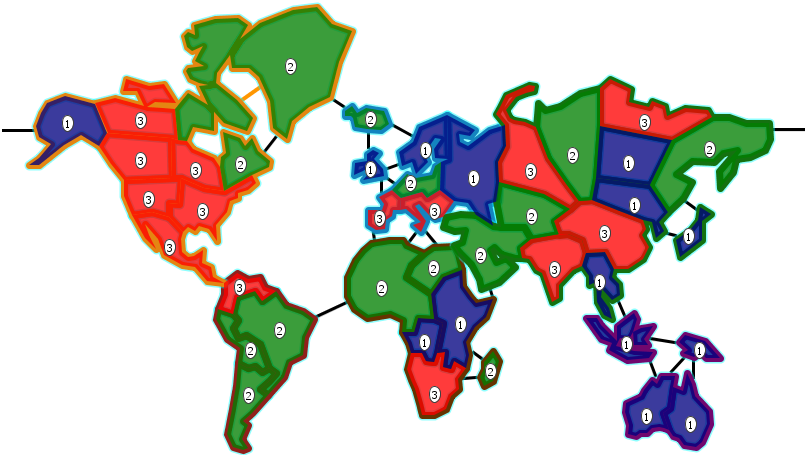
\includegraphics[scale=0.3]{../ForPublication/figs/DraftExample.png}
	\caption{An example of a draft outcome.  The territories picked by players 1, 2, and 3 are blue, green, and red respectively.  %Territories connected by a line are also considered adjacent or bordering. 
	Modified from Lux Delux.}
	\label{fig:DraftExample}
\end{figure}

\section{Empirical Evaluation}

\begin{figure*}[t]
	\centering
	\subfigure[]{
		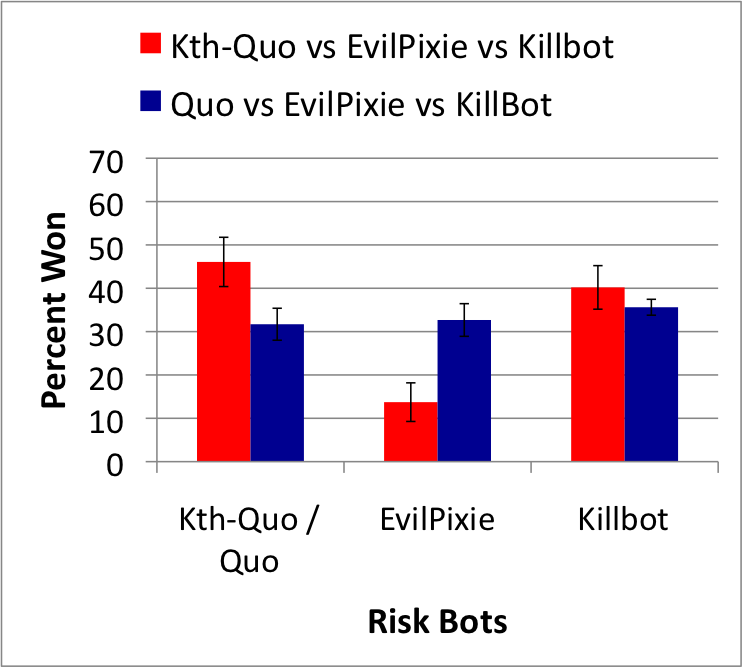
\includegraphics[scale=.4]{../ForPublication/figs/KthEvilKillBotColor.png}
		\label{fig:QuoKthEpKill}
	} %\hspace{5pt}
	\subfigure[]{
		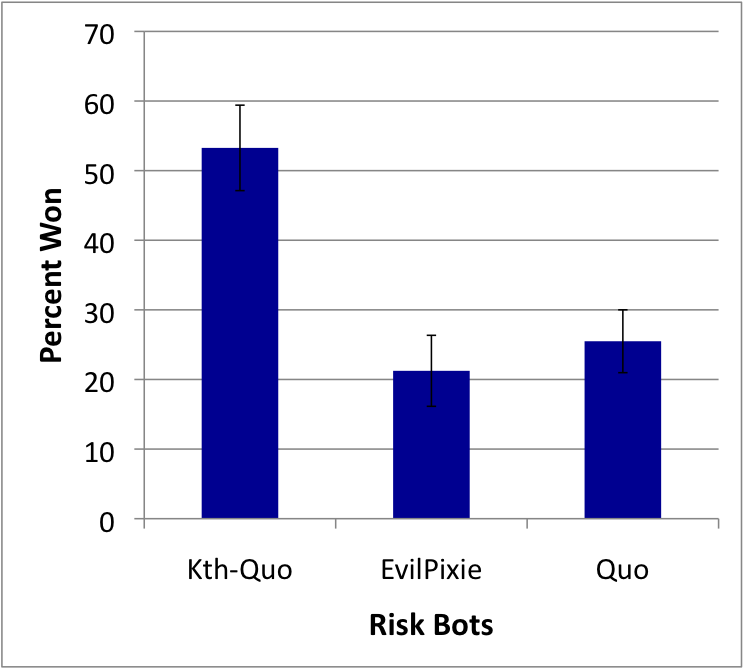
\includegraphics[scale=.4]{../ForPublication/figs/KthEvilQuoColor.png}
		\label{fig:KthQuoEvilP}
	} %\hspace{5pt}
	\subfigure[]{
		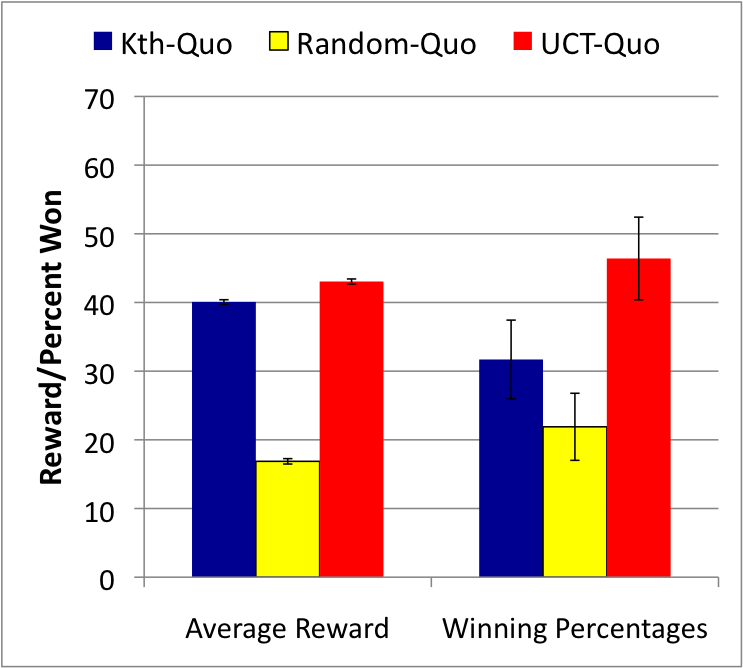
\includegraphics[scale=.4]{../ForPublication/figs/KthRandomUCTColor.png}
		\label{fig:KthUctRan}
	}
	\caption[]{Risk bot performances.  Error bars indicate 95\% confidence intervals.}
	\label{fig:RiskResults}
\end{figure*}

We created a ``UCT-Quo'' bot by replacing the drafting rules of the Quo bot provided in Lux Delux with the UCT algorithm.  The Quo bot is one of the strongest bots provided by the game, according to the game designers.  For comparison, we also created a ``Random-Quo'' and a ``Greedy-Quo'' bot that replace Quo's drafting rules with a random drafting strategy and a greedy strategy, respectively.  We ran several preliminary matches consisting of only UCT-Quo bots with different exploration parameters and found that $c=0.25$ provided the best results.  Thus, UCT-Quo used $c=0.25$ in all later experiments.  As mentioned previously, UCT-Quo ran $M = 3000$ simulations from the root decision point.  We also pitted UCT-Quo against four other existing bots in the game Lux Delux: Quo, KillBot, Boscoe and EvilPixie.

We present the experimental results in Figure \ref{fig:RiskResults}.  For each combination, the winning percentages of each bot over 50 rounds of games are reported.  Each round consisted of 6 games, one for each of the $3!$ turn orderings of the players.  All games were run with the Lux Delux settings ``selected countries'' and ``placed armies'' turned on, and ``cards'' turned off.  In addition, although Lux Delux does not automatically impose a time limit per turn, we enforced our own time limit of $750 \left \lceil \ell / 3 \right \rceil$ milliseconds, where $\ell$ equals the number of territories left to be picked.  For example, on the first turn each player has $0.75 * \left \lceil 42 / 3 \right \rceil = 10.5$ seconds to make a pick.  All experiments were run on a Pentium Dual-Core CPU 2.1 GHz with 4GB 332.5 MHz DDR2 RAM.  

The blue bars of Figure \ref{fig:QuoKthEpKill} show that Quo was equally matched against EvilPixie and Killbot, having won roughly one-third of the games against these two opponents.  However, max$^\text{n}$+UCT-Quo did significantly better than Quo against the same two opponents, having won over 50\% of the games (the red bars).  This result demonstrates that drafting territories is an important stage of Risk.

In addition, Figure \ref{fig:KthQuoEvilP} shows that despite Quo and max$^\text{n}$+UCT-Quo having the same post-draft strategy, max$^\text{n}$+UCT-Quo won nearly 65\% of its matches against Quo and EvilPixie, more than triple that of Quo.  Figures \ref{fig:QuoKthEpKill} and \ref{fig:KthQuoEvilP} together indicate that our drafting strategy significantly improves the overall performance of the Quo bot compared to using its own rule-based drafting approach.

Finally, Figure \ref{fig:KthUctRan} shows that max$^\text{n}$+UCT-Quo came first place against UCT-Quo and Random-Quo in terms of both the average draft outcome value from our machine-learned outcome evaluator (leftmost bars), and in number of wins (rightmost bars).  This suggests that for the given time limit, max$^\text{n}$+UCT is preferred over UCT for drafting Risk territories.  Furthermore, since Random-Quo wins only a small percentage of games despite having an identical post-draft strategy as its opponents, we have further evidence that the drafting phase in Risk is crucial to success.  Finally, note that the similarity in shape between the leftmost and rightmost bars shows that the draft outcome evaluator gives a decent approximation of Quo's chances of winning from the outcome.

\section{Conclusions}

% Mention video games here as future work (sports games with drafts)

% Summarize 

We presented a technique for drafting territories in the board game Risk.  Our approach combines the UCT algorithm with a machine-learned draft outcome evaluator to trim the length of each UCT simulation.  The augmented UCT-Quo bot outperformed all of the difficult bots tested within Lux Delux, including the Quo bot itself.  Our experiments indicate that the drafting stage is an important part of Risk, and combining UCT with an evaluation function is an effective computational approach for territory drafting. 

We see potential future work stemming from using UCT and a machine-learned evaluator in other types of games, particularly in other drafting-type scenarios such as in fantasy sports leagues.  Furthermore, many sports video games include a rookie or fantasy draft component and a UCT approach could provide a more intelligent opponent than current implementations.  Finally, we suspect that a more sophisticated supervised learning technique than simple linear regression may improve the performance of our Risk bot.  

%\section*{Acknowledgments}
%We would like to thank Vadim Bulitko for directing us to Lee's thesis and for suggesting Fantasy Risk.  %We would also like to thank SillySoft for providing full source code of their Risk bots in Lux Delux.

%\bibliography{../../../../LaTeX/bib}
%\bibliographystyle{../../../LaTeX/Styles/aaai}
\bibliography{bib}
\bibliographystyle{aaai}

\end{document}
